\input{header.tex}
\input{newcommands.tex}


\title{Funktionsgraphen mit \TikZ zeichnen}
\author{Fortbildungsmaterial für MINT-Lehrkräfte}
\date{\today}
\pagestyle{plain}
\setlength{\parskip}{1.5em} % Abstand zwischen Absätzen (Handreichungen)


\begin{document}

\maketitle

Funktionsgraphen gehören zu den häufigsten Abbildungen auf Mathematik-Arbeitsblättern. Damit alle Blätter einheitlich aussehen, zeigt diese Handreichung feste Vorlagen: ein Standard-Koordinatensystem und seine Varianten für Sachaufgaben, Zuordnungsaufgaben, Winkelfunktionen, Asymptoten, Flächen und Tangenten. Alle Grafiken sind mit reinem \TikZ gezeichnet, ohne \texttt{pgfplots}.



%%%%  KAPITEL 1  %%%%
\section{Das Standard-Koordinatensystem}

Alle Mathe-Arbeitsblätter verwenden dasselbe Koordinatensystem: graues Gitter, Achsen mit \texttt{-latex}-Pfeilen, Beschriftung jeder zweiten Einheit in \texttt{\textbackslash tiny}, Maßstab \texttt{scale=0.42}. Graphen stehen immer in einer \texttt{scope} mit \texttt{\textbackslash clip}, damit sie nicht über das Gitter hinauslaufen. Es wird ausschließlich reines \TikZ verwendet, kein \texttt{pgfplots}.


%%%%  UNTERKAPITEL 1.1  %%%%
\subsection{Die ausführliche Vorlage}

So sieht das Koordinatensystem ausgeschrieben aus. Diese Form ist sinnvoll, wenn man Gitter oder Achsen gezielt verändern möchte:

\begin{lstlisting}[style=latex]
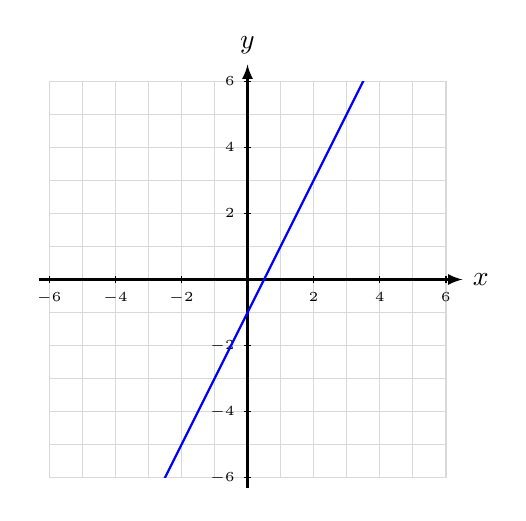
\begin{tikzpicture}[scale=0.42]
	% Gitter
	\foreach \x in {-6,...,6} \draw[gray!30, thin] (\x,-6) -- (\x,6);
	\foreach \y in {-6,...,6} \draw[gray!30, thin] (-6,\y) -- (6,\y);
	% Achsen
	\draw[-latex, thick] (-6.3,0) -- (6.5,0) node[right] {$x$};
	\draw[-latex, thick] (0,-6.3) -- (0,6.5) node[above] {$y$};
	% Beschriftung
	\foreach \x in {-6,-4,-2,2,4,6}
		\draw (\x,0.1) -- (\x,-0.1) node[below, font=\tiny] {$\x$};
	\foreach \y in {-6,-4,-2,2,4,6}
		\draw (0.1,\y) -- (-0.1,\y) node[left, font=\tiny] {$\y$};
	% Graph – immer in einer clip-scope
	\begin{scope}
		\clip (-6,-6) rectangle (6,6);
		\draw[blue, thick, domain=-6:6, samples=200] plot (\x, {2*\x - 1});
	\end{scope}
\end{tikzpicture}
\end{lstlisting}

\begin{ausgabe}
\centering
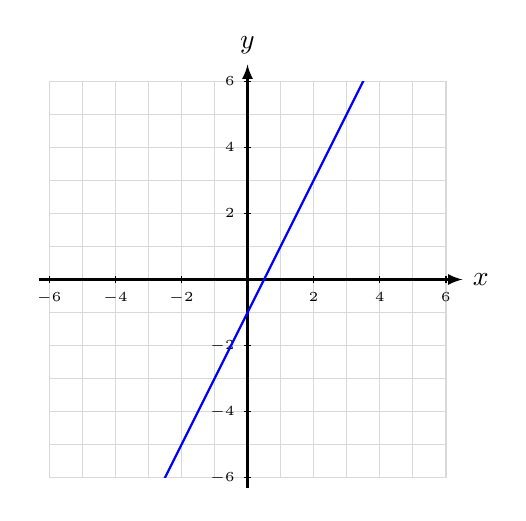
\begin{tikzpicture}[scale=0.42]
	% Gitter
	\foreach \x in {-6,...,6} \draw[gray!30, thin] (\x,-6) -- (\x,6);
	\foreach \y in {-6,...,6} \draw[gray!30, thin] (-6,\y) -- (6,\y);
	% Achsen
	\draw[-latex, thick] (-6.3,0) -- (6.5,0) node[right] {$x$};
	\draw[-latex, thick] (0,-6.3) -- (0,6.5) node[above] {$y$};
	% Beschriftung
	\foreach \x in {-6,-4,-2,2,4,6}
		\draw (\x,0.1) -- (\x,-0.1) node[below, font=\tiny] {$\x$};
	\foreach \y in {-6,-4,-2,2,4,6}
		\draw (0.1,\y) -- (-0.1,\y) node[left, font=\tiny] {$\y$};
	% Graph – immer in einer clip-scope
	\begin{scope}
		\clip (-6,-6) rectangle (6,6);
		\draw[blue, thick, domain=-6:6, samples=200] plot (\x, {2*\x - 1});
	\end{scope}
\end{tikzpicture}
\end{ausgabe}


%%%%  UNTERKAPITEL 1.2  %%%%
\subsection{Kurzform mit \texttt{\textbackslash koordinatensystem}}

In der universalen \texttt{newcommands.tex} steht der Befehl \texttt{\textbackslash koordinatensystem}. Er erwartet den optionalen Beschriftungsschritt und vier ganze Zahlen: \texttt{[Schritt]\{xmin\}\{xmax\}\{ymin\}\{ymax\}}. Er zeichnet Gitter, Achsen und Beschriftung genau wie die ausführliche Vorlage. Der optionale Schritt (Standard 2) legt fest, welche Zahlen an den Achsen stehen:

\begin{lstlisting}[style=latex]
\begin{tikzpicture}[scale=0.42]
	\koordinatensystem{-6}{6}{-6}{6}
	\begin{scope}
		\clip (-6,-6) rectangle (6,6);
		\draw[blue, thick, domain=-6:6, samples=200] plot (\x, {2*\x - 1});
	\end{scope}
	\node[blue, font=\scriptsize] at (4.2,5.4) {$f$};
\end{tikzpicture}
\end{lstlisting}

\begin{ausgabe}
\centering
\begin{tikzpicture}[scale=0.42]
	\koordinatensystem{-6}{6}{-6}{6}
	\begin{scope}
		\clip (-6,-6) rectangle (6,6);
		\draw[blue, thick, domain=-6:6, samples=200] plot (\x, {2*\x - 1});
	\end{scope}
	\node[blue, font=\scriptsize] at (4.2,5.4) {$f$};
\end{tikzpicture}
\end{ausgabe}

Die Funktionsbeschriftung steht in der Farbe des Graphen in \texttt{\textbackslash scriptsize} an einer freien Stelle nahe dem Graphen.



%%%%  KAPITEL 2  %%%%
\section{Mehrere Funktionen und Punkte}


%%%%  UNTERKAPITEL 2.1  %%%%
\subsection{Mehrere Graphen in einem Koordinatensystem}

Für mehrere Graphen werden die Farben in dieser Reihenfolge verwendet: \texttt{blue}, \texttt{red}, \texttt{green!60!black}, \texttt{orange}. Potenzen negativer Zahlen immer klammern: \texttt{(\textbackslash x)\^{}2}.

\begin{lstlisting}[style=latex]
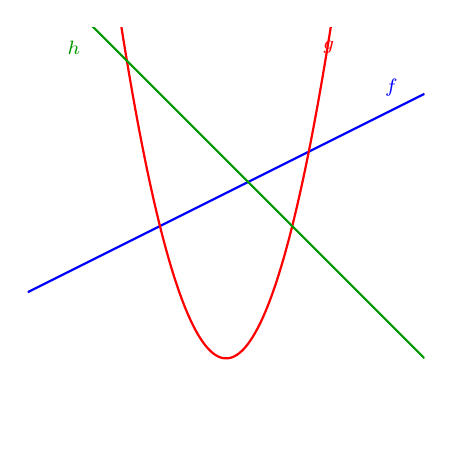
\begin{tikzpicture}[scale=0.42]
	\koordinatensystem{-6}{6}{-6}{6}
	\begin{scope}
		\clip (-6,-6) rectangle (6,6);
		\draw[blue, thick, domain=-6:6, samples=200] plot (\x, {0.5*\x + 1});
		\draw[red, thick, domain=-6:6, samples=200] plot (\x, {(\x)^2 - 4});
		\draw[green!60!black, thick, domain=-6:6, samples=200] plot (\x, {-\x + 2});
	\end{scope}
	\node[blue, font=\scriptsize] at (5,4.2) {$f$};
	\node[red, font=\scriptsize] at (3.1,5.4) {$g$};
	\node[green!60!black, font=\scriptsize] at (-4.6,5.4) {$h$};
\end{tikzpicture}
\end{lstlisting}

\begin{ausgabe}
\centering
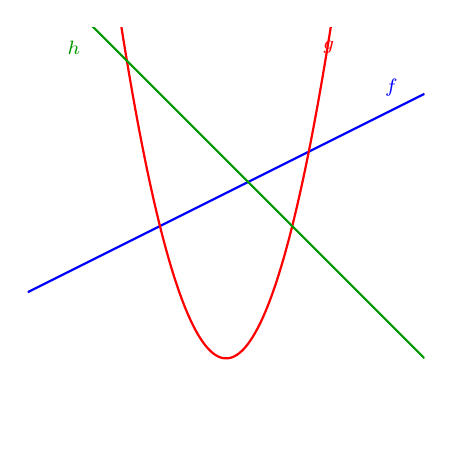
\begin{tikzpicture}[scale=0.42]
	\koordinatensystem{-6}{6}{-6}{6}
	\begin{scope}
		\clip (-6,-6) rectangle (6,6);
		\draw[blue, thick, domain=-6:6, samples=200] plot (\x, {0.5*\x + 1});
		\draw[red, thick, domain=-6:6, samples=200] plot (\x, {(\x)^2 - 4});
		\draw[green!60!black, thick, domain=-6:6, samples=200] plot (\x, {-\x + 2});
	\end{scope}
	\node[blue, font=\scriptsize] at (5,4.2) {$f$};
	\node[red, font=\scriptsize] at (3.1,5.4) {$g$};
	\node[green!60!black, font=\scriptsize] at (-4.6,5.4) {$h$};
\end{tikzpicture}
\end{ausgabe}


%%%%  UNTERKAPITEL 2.2  %%%%
\subsection{Punkte markieren und beschriften}

Punkte werden mit dem Stil \texttt{punkt} als Knoten gesetzt. So bleiben sie auch bei \texttt{scale=0.42} gut sichtbar; ein \texttt{circle (3pt)} würde mitverkleinert.

\begin{lstlisting}[style=latex]
\begin{tikzpicture}[scale=0.42]
	\koordinatensystem{-6}{6}{-6}{6}
	\begin{scope}
		\clip (-6,-6) rectangle (6,6);
		\draw[blue, thick, domain=-6:6, samples=200] plot (\x, {0.5*(\x)^2 - 2});
		\draw[red, thick, domain=-6:6, samples=200] plot (\x, {\x + 2});
	\end{scope}
	% Schnittpunkte von f und g
	\node[punkt, label={[font=\scriptsize]left:$S_1(-2\mid 0)$}] at (-2,0) {};
	\node[punkt, label={[font=\scriptsize]right:$S_2(4\mid 6)$}] at (4,6) {};
	% Scheitelpunkt
	\node[punkt, label={[font=\scriptsize]below right:$S(0\mid -2)$}] at (0,-2) {};
\end{tikzpicture}
\end{lstlisting}

\begin{ausgabe}
\centering
\begin{tikzpicture}[scale=0.42]
	\koordinatensystem{-6}{6}{-6}{6}
	\begin{scope}
		\clip (-6,-6) rectangle (6,6);
		\draw[blue, thick, domain=-6:6, samples=200] plot (\x, {0.5*(\x)^2 - 2});
		\draw[red, thick, domain=-6:6, samples=200] plot (\x, {\x + 2});
	\end{scope}
	% Schnittpunkte von f und g
	\node[punkt, label={[font=\scriptsize]left:$S_1(-2\mid 0)$}] at (-2,0) {};
	\node[punkt, label={[font=\scriptsize]right:$S_2(4\mid 6)$}] at (4,6) {};
	% Scheitelpunkt
	\node[punkt, label={[font=\scriptsize]below right:$S(0\mid -2)$}] at (0,-2) {};
\end{tikzpicture}
\end{ausgabe}



%%%%  KAPITEL 3  %%%%
\section{Varianten des Koordinatensystems}


%%%%  UNTERKAPITEL 3.1  %%%%
\subsection{Sachaufgaben im ersten Quadranten}

Bei Sachaufgaben stehen an den Achsen Größe und Einheit. Das Gitter beginnt bei null:

\begin{lstlisting}[style=latex]
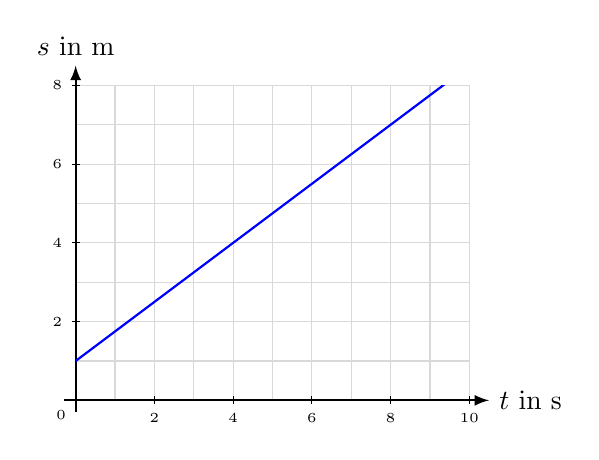
\begin{tikzpicture}[scale=0.5]
	% Gitter im 1. Quadranten, Achsen mit Größe und Einheit
	\foreach \x in {0,...,10} \draw[gray!30, thin] (\x,0) -- (\x,8);
	\foreach \y in {0,...,8} \draw[gray!30, thin] (0,\y) -- (10,\y);
	\draw[-latex, thick] (-0.3,0) -- (10.5,0) node[right] {$t$ in s};
	\draw[-latex, thick] (0,-0.3) -- (0,8.5) node[above] {$s$ in m};
	\foreach \x in {2,4,...,10}
		\draw (\x,0.1) -- (\x,-0.1) node[below, font=\tiny] {$\x$};
	\foreach \y in {2,4,...,8}
		\draw (0.1,\y) -- (-0.1,\y) node[left, font=\tiny] {$\y$};
	\node[below left, font=\tiny] at (0,0) {$0$};
	\begin{scope}
		\clip (0,0) rectangle (10,8);
		\draw[blue, thick, domain=0:10, samples=200] plot (\x, {0.75*\x + 1});
	\end{scope}
\end{tikzpicture}
\end{lstlisting}

\begin{ausgabe}
\centering
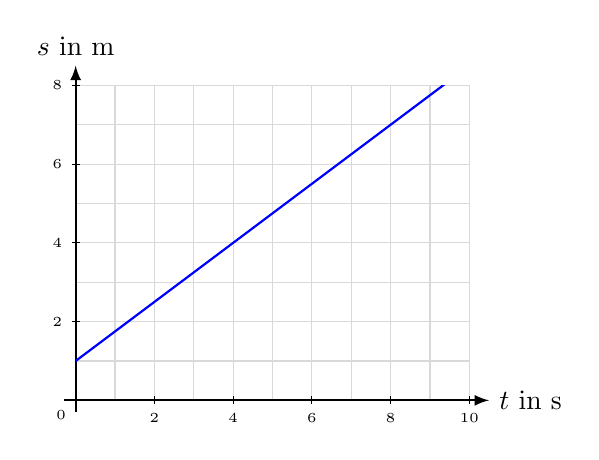
\begin{tikzpicture}[scale=0.5]
	% Gitter im 1. Quadranten, Achsen mit Größe und Einheit
	\foreach \x in {0,...,10} \draw[gray!30, thin] (\x,0) -- (\x,8);
	\foreach \y in {0,...,8} \draw[gray!30, thin] (0,\y) -- (10,\y);
	\draw[-latex, thick] (-0.3,0) -- (10.5,0) node[right] {$t$ in s};
	\draw[-latex, thick] (0,-0.3) -- (0,8.5) node[above] {$s$ in m};
	\foreach \x in {2,4,...,10}
		\draw (\x,0.1) -- (\x,-0.1) node[below, font=\tiny] {$\x$};
	\foreach \y in {2,4,...,8}
		\draw (0.1,\y) -- (-0.1,\y) node[left, font=\tiny] {$\y$};
	\node[below left, font=\tiny] at (0,0) {$0$};
	\begin{scope}
		\clip (0,0) rectangle (10,8);
		\draw[blue, thick, domain=0:10, samples=200] plot (\x, {0.75*\x + 1});
	\end{scope}
\end{tikzpicture}
\end{ausgabe}


%%%%  UNTERKAPITEL 3.2  %%%%
\subsection{Drei Graphen nebeneinander}

Für Zuordnungsaufgaben stehen drei kleinere Koordinatensysteme mit \texttt{scale=0.52} nebeneinander:

\begin{lstlisting}[style=latex]
\begin{tikzpicture}[scale=0.52]
	\koordinatensystem{-4}{4}{-4}{4}
	\begin{scope}
		\clip (-4,-4) rectangle (4,4);
		\draw[blue, thick, domain=-4:4, samples=200] plot (\x, {(\x)^2 - 3});
	\end{scope}
	\node[font=\scriptsize] at (-3,3.4) {(A)};
\end{tikzpicture}
\hfill
\begin{tikzpicture}[scale=0.52]
	\koordinatensystem{-4}{4}{-4}{4}
	\begin{scope}
		\clip (-4,-4) rectangle (4,4);
		\draw[blue, thick, domain=-4:4, samples=200] plot (\x, {-(\x-1)^2 + 2});
	\end{scope}
	\node[font=\scriptsize] at (-3,3.4) {(B)};
\end{tikzpicture}
\hfill
\begin{tikzpicture}[scale=0.52]
	\koordinatensystem{-4}{4}{-4}{4}
	\begin{scope}
		\clip (-4,-4) rectangle (4,4);
		\draw[blue, thick, domain=-4:4, samples=200] plot (\x, {0.5*(\x+1)^2 - 2});
	\end{scope}
	\node[font=\scriptsize] at (-3,3.4) {(C)};
\end{tikzpicture}
\end{lstlisting}

\begin{ausgabe}
\centering
\begin{tikzpicture}[scale=0.52]
	\koordinatensystem{-4}{4}{-4}{4}
	\begin{scope}
		\clip (-4,-4) rectangle (4,4);
		\draw[blue, thick, domain=-4:4, samples=200] plot (\x, {(\x)^2 - 3});
	\end{scope}
	\node[font=\scriptsize] at (-3,3.4) {(A)};
\end{tikzpicture}
\hfill
\begin{tikzpicture}[scale=0.52]
	\koordinatensystem{-4}{4}{-4}{4}
	\begin{scope}
		\clip (-4,-4) rectangle (4,4);
		\draw[blue, thick, domain=-4:4, samples=200] plot (\x, {-(\x-1)^2 + 2});
	\end{scope}
	\node[font=\scriptsize] at (-3,3.4) {(B)};
\end{tikzpicture}
\hfill
\begin{tikzpicture}[scale=0.52]
	\koordinatensystem{-4}{4}{-4}{4}
	\begin{scope}
		\clip (-4,-4) rectangle (4,4);
		\draw[blue, thick, domain=-4:4, samples=200] plot (\x, {0.5*(\x+1)^2 - 2});
	\end{scope}
	\node[font=\scriptsize] at (-3,3.4) {(C)};
\end{tikzpicture}
\end{ausgabe}


%%%%  UNTERKAPITEL 3.3  %%%%
\subsection{Trigonometrische Funktionen}

Bei Winkelfunktionen wird die $x$-Achse in Vielfachen von $\frac{\pi}{2}$ beschriftet. Wichtig: \TikZ rechnet in Grad. Für das Bogenmaß steht ein \texttt{r} hinter dem Argument: \texttt{sin(\textbackslash x r)}.

\begin{lstlisting}[style=latex]
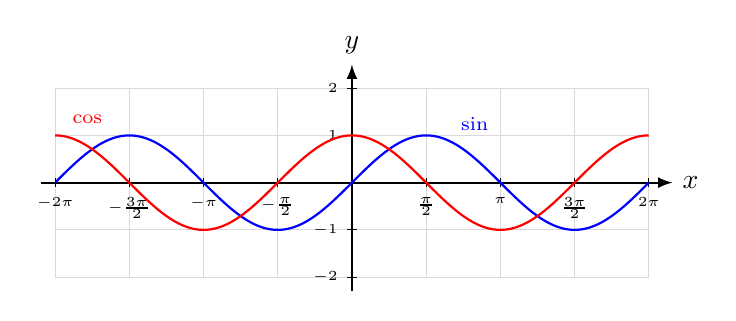
\begin{tikzpicture}[scale=0.6]
	% Gitter: senkrecht bei Vielfachen von pi/2, waagerecht bei ganzen Zahlen
	\foreach \k in {-4,...,4} \draw[gray!30, thin] ({\k*pi/2},-2) -- ({\k*pi/2},2);
	\foreach \y in {-2,...,2} \draw[gray!30, thin] ({-2*pi},\y) -- ({2*pi},\y);
	\draw[-latex, thick] ({-2*pi-0.3},0) -- ({2*pi+0.5},0) node[right] {$x$};
	\draw[-latex, thick] (0,-2.3) -- (0,2.5) node[above] {$y$};
	\foreach \k/\t in {-4/-2\pi, -3/-\frac{3\pi}{2}, -2/-\pi, -1/-\frac{\pi}{2},
	                   1/\frac{\pi}{2}, 2/\pi, 3/\frac{3\pi}{2}, 4/2\pi}
		\draw ({\k*pi/2},0.1) -- ({\k*pi/2},-0.1) node[below, font=\tiny] {$\t$};
	\foreach \y in {-2,-1,1,2}
		\draw (0.1,\y) -- (-0.1,\y) node[left, font=\tiny] {$\y$};
	\begin{scope}
		\clip ({-2*pi},-2) rectangle ({2*pi},2);
		% Bogenmaß: r hinter dem Argument!
		\draw[blue, thick, domain={-2*pi}:{2*pi}, samples=200] plot (\x, {sin(\x r)});
		\draw[red, thick, domain={-2*pi}:{2*pi}, samples=200] plot (\x, {cos(\x r)});
	\end{scope}
	\node[blue, font=\scriptsize] at (2.6,1.25) {$\sin$};
	\node[red, font=\scriptsize] at (-5.6,1.35) {$\cos$};
\end{tikzpicture}
\end{lstlisting}

\begin{ausgabe}
\centering
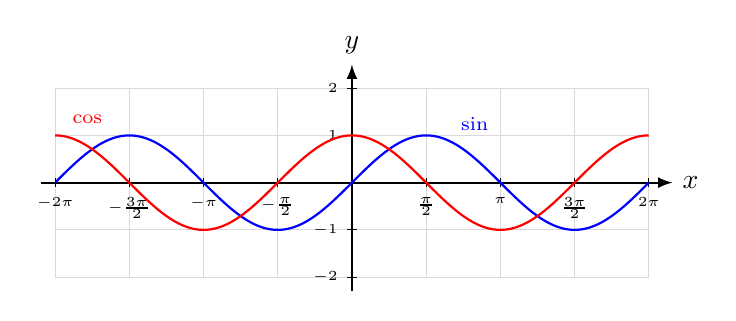
\begin{tikzpicture}[scale=0.6]
	% Gitter: senkrecht bei Vielfachen von pi/2, waagerecht bei ganzen Zahlen
	\foreach \k in {-4,...,4} \draw[gray!30, thin] ({\k*pi/2},-2) -- ({\k*pi/2},2);
	\foreach \y in {-2,...,2} \draw[gray!30, thin] ({-2*pi},\y) -- ({2*pi},\y);
	\draw[-latex, thick] ({-2*pi-0.3},0) -- ({2*pi+0.5},0) node[right] {$x$};
	\draw[-latex, thick] (0,-2.3) -- (0,2.5) node[above] {$y$};
	\foreach \k/\t in {-4/-2\pi, -3/-\frac{3\pi}{2}, -2/-\pi, -1/-\frac{\pi}{2},
	                   1/\frac{\pi}{2}, 2/\pi, 3/\frac{3\pi}{2}, 4/2\pi}
		\draw ({\k*pi/2},0.1) -- ({\k*pi/2},-0.1) node[below, font=\tiny] {$\t$};
	\foreach \y in {-2,-1,1,2}
		\draw (0.1,\y) -- (-0.1,\y) node[left, font=\tiny] {$\y$};
	\begin{scope}
		\clip ({-2*pi},-2) rectangle ({2*pi},2);
		% Bogenmaß: r hinter dem Argument!
		\draw[blue, thick, domain={-2*pi}:{2*pi}, samples=200] plot (\x, {sin(\x r)});
		\draw[red, thick, domain={-2*pi}:{2*pi}, samples=200] plot (\x, {cos(\x r)});
	\end{scope}
	\node[blue, font=\scriptsize] at (2.6,1.25) {$\sin$};
	\node[red, font=\scriptsize] at (-5.6,1.35) {$\cos$};
\end{tikzpicture}
\end{ausgabe}



%%%%  KAPITEL 4  %%%%
\section{Besondere Funktionstypen}


%%%%  UNTERKAPITEL 4.1  %%%%
\subsection{Gebrochen-rationale Funktionen mit Asymptoten}

An einer Polstelle wird der Definitionsbereich in zwei Äste geteilt; die Asymptoten werden grau gestrichelt:

\begin{lstlisting}[style=latex]
\begin{tikzpicture}[scale=0.42]
	\koordinatensystem{-6}{6}{-6}{6}
	% Asymptoten gestrichelt
	\draw[dashed, gray] (1,-6) -- (1,6);
	\draw[dashed, gray] (-6,2) -- (6,2);
	\begin{scope}
		\clip (-6,-6) rectangle (6,6);
		% zwei Äste: Polstelle x = 1 aus dem Definitionsbereich herausnehmen
		\draw[blue, thick, domain=-6:0.87, samples=200] plot (\x, {1/(\x-1) + 2});
		\draw[blue, thick, domain=1.13:6, samples=200] plot (\x, {1/(\x-1) + 2});
	\end{scope}
	\node[gray, font=\scriptsize] at (1.9,-5.4) {$x=1$};
	\node[gray, font=\scriptsize] at (-5,2.6) {$y=2$};
\end{tikzpicture}
\end{lstlisting}

\begin{ausgabe}
\centering
\begin{tikzpicture}[scale=0.42]
	\koordinatensystem{-6}{6}{-6}{6}
	% Asymptoten gestrichelt
	\draw[dashed, gray] (1,-6) -- (1,6);
	\draw[dashed, gray] (-6,2) -- (6,2);
	\begin{scope}
		\clip (-6,-6) rectangle (6,6);
		% zwei Äste: Polstelle x = 1 aus dem Definitionsbereich herausnehmen
		\draw[blue, thick, domain=-6:0.87, samples=200] plot (\x, {1/(\x-1) + 2});
		\draw[blue, thick, domain=1.13:6, samples=200] plot (\x, {1/(\x-1) + 2});
	\end{scope}
	\node[gray, font=\scriptsize] at (1.9,-5.4) {$x=1$};
	\node[gray, font=\scriptsize] at (-5,2.6) {$y=2$};
\end{tikzpicture}
\end{ausgabe}


%%%%  UNTERKAPITEL 4.2  %%%%
\subsection{Exponentialfunktionen}

Potenzen mit variablem Exponenten schreibt man \texttt{2\^{}(\textbackslash x)}, die e-Funktion als \texttt{exp(\textbackslash x)}:

\begin{lstlisting}[style=latex]
\begin{tikzpicture}[scale=0.42]
	\koordinatensystem{-6}{6}{-2}{8}
	\begin{scope}
		\clip (-6,-2) rectangle (6,8);
		\draw[blue, thick, domain=-6:6, samples=200] plot (\x, {2^(\x)});
		\draw[red, thick, domain=-6:6, samples=200] plot (\x, {exp(-\x)});
	\end{scope}
	\node[punkt, label={[font=\scriptsize]right:$(0\mid 1)$}] at (0,1) {};
	\node[blue, font=\scriptsize] at (3.6,7) {$f(x)=2^x$};
	\node[red, font=\scriptsize] at (-4.6,7) {$g(x)=\mathrm{e}^{-x}$};
\end{tikzpicture}
\end{lstlisting}

\begin{ausgabe}
\centering
\begin{tikzpicture}[scale=0.42]
	\koordinatensystem{-6}{6}{-2}{8}
	\begin{scope}
		\clip (-6,-2) rectangle (6,8);
		\draw[blue, thick, domain=-6:6, samples=200] plot (\x, {2^(\x)});
		\draw[red, thick, domain=-6:6, samples=200] plot (\x, {exp(-\x)});
	\end{scope}
	\node[punkt, label={[font=\scriptsize]right:$(0\mid 1)$}] at (0,1) {};
	\node[blue, font=\scriptsize] at (3.6,7) {$f(x)=2^x$};
	\node[red, font=\scriptsize] at (-4.6,7) {$g(x)=\mathrm{e}^{-x}$};
\end{tikzpicture}
\end{ausgabe}


%%%%  UNTERKAPITEL 4.3  %%%%
\subsection{Abschnittsweise definierte Funktionen}

Ein voller Punkt gehört zum Graphen, ein offener Punkt (Stil \texttt{punktoffen}) nicht:

\begin{lstlisting}[style=latex]
\begin{tikzpicture}[scale=0.42]
	\koordinatensystem{-6}{6}{-6}{6}
	\begin{scope}
		\clip (-6,-6) rectangle (6,6);
		\draw[blue, thick, domain=-6:2, samples=200] plot (\x, {0.5*\x + 1});
		\draw[blue, thick, domain=2:6, samples=200] plot (\x, {-\x + 6});
	\end{scope}
	% gehört dazu: voller Punkt, gehört nicht dazu: offener Punkt
	\node[punkt, blue] at (2,2) {};
	\node[punktoffen, draw=blue] at (2,4) {};
\end{tikzpicture}
\end{lstlisting}

\begin{ausgabe}
\centering
\begin{tikzpicture}[scale=0.42]
	\koordinatensystem{-6}{6}{-6}{6}
	\begin{scope}
		\clip (-6,-6) rectangle (6,6);
		\draw[blue, thick, domain=-6:2, samples=200] plot (\x, {0.5*\x + 1});
		\draw[blue, thick, domain=2:6, samples=200] plot (\x, {-\x + 6});
	\end{scope}
	% gehört dazu: voller Punkt, gehört nicht dazu: offener Punkt
	\node[punkt, blue] at (2,2) {};
	\node[punktoffen, draw=blue] at (2,4) {};
\end{tikzpicture}
\end{ausgabe}



%%%%  KAPITEL 5  %%%%
\section{Analysis}


%%%%  UNTERKAPITEL 5.1  %%%%
\subsection{Fläche unter einem Graphen}

Die Fläche wird als geschlossener Pfad gefüllt: Punkt auf der $x$-Achse, entlang des Graphen, zurück zur $x$-Achse. Erst füllen, dann den Graphen darüber zeichnen:

\begin{lstlisting}[style=latex]
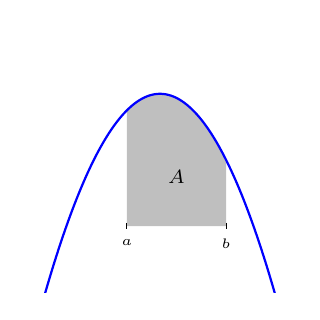
\begin{tikzpicture}[scale=0.42]
	\koordinatensystem{-2}{6}{-2}{6}
	\begin{scope}
		\clip (-2,-2) rectangle (6,6);
		% Fläche zwischen Graph und x-Achse von a = 1 bis b = 4
		\fill[gray, opacity=0.5] (1,0) -- plot[domain=1:4, samples=100] (\x, {-0.5*(\x-2)^2 + 4}) -- (4,0) -- cycle;
		\draw[blue, thick, domain=-2:6, samples=200] plot (\x, {-0.5*(\x-2)^2 + 4});
	\end{scope}
	\draw (1,0.1) -- (1,-0.1) node[below, font=\tiny] {$a$};
	\draw (4,0.1) -- (4,-0.1) node[below, font=\tiny] {$b$};
	\node[font=\scriptsize] at (2.5,1.5) {$A$};
\end{tikzpicture}
\end{lstlisting}

\begin{ausgabe}
\centering
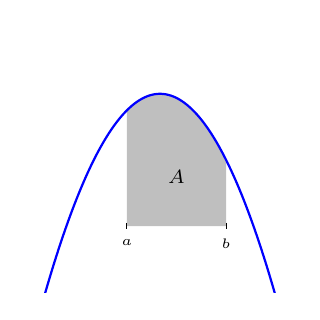
\begin{tikzpicture}[scale=0.42]
	\koordinatensystem{-2}{6}{-2}{6}
	\begin{scope}
		\clip (-2,-2) rectangle (6,6);
		% Fläche zwischen Graph und x-Achse von a = 1 bis b = 4
		\fill[gray, opacity=0.5] (1,0) -- plot[domain=1:4, samples=100] (\x, {-0.5*(\x-2)^2 + 4}) -- (4,0) -- cycle;
		\draw[blue, thick, domain=-2:6, samples=200] plot (\x, {-0.5*(\x-2)^2 + 4});
	\end{scope}
	\draw (1,0.1) -- (1,-0.1) node[below, font=\tiny] {$a$};
	\draw (4,0.1) -- (4,-0.1) node[below, font=\tiny] {$b$};
	\node[font=\scriptsize] at (2.5,1.5) {$A$};
\end{tikzpicture}
\end{ausgabe}


%%%%  UNTERKAPITEL 5.2  %%%%
\subsection{Tangente an einen Graphen}

Die Tangente wird als lineare Funktion berechnet und wie ein Graph gezeichnet; der Berührpunkt bekommt einen Punkt:

\begin{lstlisting}[style=latex]
\begin{tikzpicture}[scale=0.42]
	\koordinatensystem{-6}{6}{-6}{6}
	\begin{scope}
		\clip (-6,-6) rectangle (6,6);
		\draw[blue, thick, domain=-6:6, samples=200] plot (\x, {0.5*(\x)^2 - 2});
		% Tangente in x0 = 2: t(x) = f'(2)(x - 2) + f(2) = 2x - 4
		\draw[red, thick, domain=-6:6] plot (\x, {2*\x - 4});
	\end{scope}
	\node[punkt, label={[font=\scriptsize]right:$P(2\mid 0)$}] at (2,0) {};
	\node[blue, font=\scriptsize] at (-4.4,5.4) {$f$};
	\node[red, font=\scriptsize] at (5.2,4.4) {$t$};
\end{tikzpicture}
\end{lstlisting}

\begin{ausgabe}
\centering
\begin{tikzpicture}[scale=0.42]
	\koordinatensystem{-6}{6}{-6}{6}
	\begin{scope}
		\clip (-6,-6) rectangle (6,6);
		\draw[blue, thick, domain=-6:6, samples=200] plot (\x, {0.5*(\x)^2 - 2});
		% Tangente in x0 = 2: t(x) = f'(2)(x - 2) + f(2) = 2x - 4
		\draw[red, thick, domain=-6:6] plot (\x, {2*\x - 4});
	\end{scope}
	\node[punkt, label={[font=\scriptsize]right:$P(2\mid 0)$}] at (2,0) {};
	\node[blue, font=\scriptsize] at (-4.4,5.4) {$f$};
	\node[red, font=\scriptsize] at (5.2,4.4) {$t$};
\end{tikzpicture}
\end{ausgabe}



%%%%  KAPITEL 6  %%%%
\section{Zusammenfassung}

Die wichtigsten Regeln für Funktionsgraphen:

\begin{itemize}
	\item Koordinatensystem mit \texttt{\textbackslash koordinatensystem} oder der ausführlichen Vorlage, Maßstab \texttt{scale=0.42} (drei nebeneinander: \texttt{0.52})
	\item Graphen immer in \texttt{\textbackslash begin\{scope\}\textbackslash clip \dots\textbackslash end\{scope\}}
	\item \texttt{samples=200} für glatte Kurven, Potenzen negativer Zahlen klammern: \texttt{(\textbackslash x)\^{}2}
	\item Bogenmaß mit \texttt{r}: \texttt{sin(\textbackslash x r)}
	\item Punkte mit dem Stil \texttt{punkt} bzw. \texttt{punktoffen}, Beschriftung in \texttt{\textbackslash scriptsize}
	\item Farben in der Reihenfolge blau, rot, grün, orange
\end{itemize}

Mit diesen Vorlagen entstehen Arbeitsblätter, auf denen alle Graphen gleich aussehen. Schülerinnen und Schüler finden sich dadurch schneller zurecht und können sich auf die Mathematik konzentrieren.

\end{document}
